% \appendix

% 📘 appendix-A5-mimo-and-beamforming-simulation.tex

\chapter{Appendix: MIMO \& Beamforming Simulation}

\section{MIMO \& Beamforming Simulation}

\subsection{Overview}
This appendix supplements Chapter 5 by providing simulation code and interactive visualizations to reinforce understanding of key MIMO and beamforming concepts.

\subsection{Jupyter Notebook: MIMO and Beamforming Simulation}

The notebook \texttt{A5\_mimo\_beamforming\_simulation.ipynb} covers the following topics:

\begin{itemize}
    \item Simulation of a MIMO channel
    \item Calculation of MIMO channel capacity
    \item Beamforming weight computation
    \item Visualization of antenna beam patterns
    \item Exploration of capacity scaling with antenna count
\end{itemize}

\noindent\textbf{Download notebook:} \\
\url{https://your-download-link.com/A5_mimo_beamforming_simulation.ipynb} \hfill (replace with actual link)

\begin{figure}[h!]
    \centering
    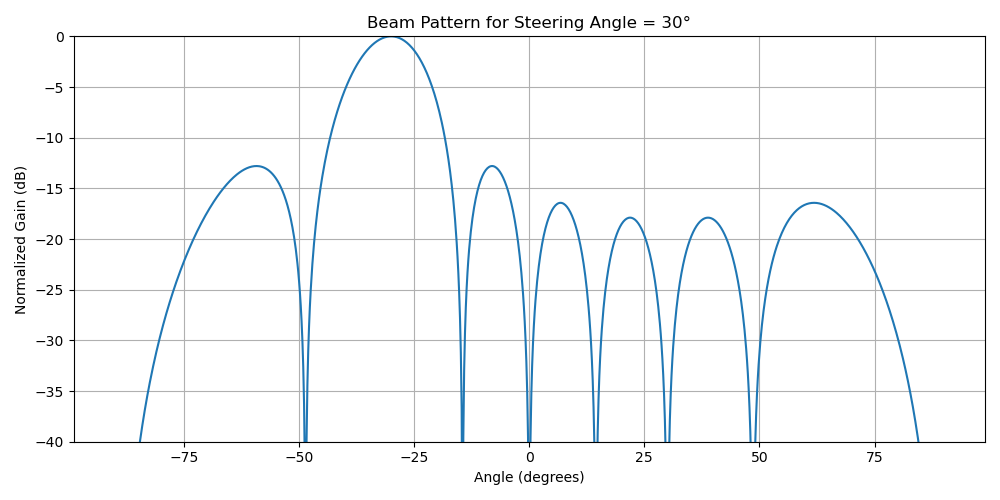
\includegraphics[width=0.9\textwidth]{./figures/beam_pattern_example.png}
    \caption{Example beam pattern for an 8-element uniform linear array steering at $30^\circ$}
    \label{fig:beam-pattern}
\end{figure}

\subsection{Interactive Streamlit App: Beam Pattern Visualizer}

An interactive app named \texttt{BeamPatternVisualizer.py} allows students to explore beamforming characteristics in real time.

\begin{itemize}
    \item Select number of antennas and spacing
    \item Adjust steering direction
    \item Switch between analog, digital, and hybrid beamforming
\end{itemize}

\noindent\textbf{Run app:} \\
\url{https://your-streamlit-link.com/BeamPatternVisualizer} \hfill (replace with actual deployed URL)

\subsection{Key Learnings}

\begin{itemize}
    \item Increasing the number of antennas enhances directionality and capacity
    \item Beamforming focuses signal energy toward desired directions
    \item Analog beamforming uses phase shifts only, while digital uses complex weights
    \item Hybrid beamforming provides a practical trade-off
\end{itemize}

\subsection{References}

\begin{itemize}
    \item T. L. Marzetta, ``Noncooperative Cellular Wireless with Unlimited Numbers of Base Station Antennas,'' IEEE Trans. Wireless Commun., 2010.
    \item A. Goldsmith, ``Wireless Communications,'' Cambridge University Press, 2005.
    \item D. Tse and P. Viswanath, ``Fundamentals of Wireless Communication,'' Cambridge University Press.
\end{itemize}
